\externaldocument{../3/chapter_modeling}
\externaldocument{../4/chapter_algorithm}
\startchapter{Feature Prototype On Atlantis}
\label{chapter:newsol}
In this section, I describe the design of the feature prototype of communication identification from the dual\_trace. This feature is implemented on Atlantis and is built on top of Atlantis' other features, such as ``memory reconstruction", ``function inspect" and ``views synchronization". Atlantis is an assembly trace analysis environment. It provides many powerful and novel features to assist assembly level execution trace analysis.\cite{huang2017atlantis} This prototype implemented the algorithms described in Chapter\ref{chapter:alo} as well as the user interfaces for the feature.

This prototype consist of four main components: 1) user defined setting for defining the concerned communication methods' function set. 2) a view that can parallelly present both traces in the dual\_trace. 3) two identification features: Stream identification and communication identification. 4) functionality that allow user to access the identification result.


\section{User Defined Function Set}\label{functionset}
As emphasized in Section\ref{windows}, the function set for each communication method can be different depends on the implementation solution of the method. Furthermore, there are so many communication methods in the real world and not all of them are being analyzed by the user. Instead of using hard coded function sets, a configuration file in Json format is used for the users to define their concerned communication methods and the corresponding function set. This function sets will be the input for the communication identification. All concerned communication methods have its own function set. The identification features implemented in this prototype iterate all methods in the Json configuration file named ``communicationMethods.json" and identify all communications of each method. This configuration includes the communication method, their function set for the communication events and the essential parameters of each function. A default template is given for user reference, this default template is generated by Atlantis when it was launched and stored in the .tmp folder in the trace analysis project folder. The default template example can be find in Section\ref{funcset}.

\section{Parallel Editor View For Dual\_Trace}
The dual\_trace consist of two execution traces which are interacting with each other. Presenting them in the same view makes the analysis for the user much easier. The strategy to open parallel editor view is that open one trace as the normal one and the other as the dual\_trace of the current opened one. A new menu option in the project navigation view are created to open the second trace as the dual\_trace of the current active trace. The implementation of the parallel editor take the advantage of the existing SWT of Eclipse plug-in development. The detail of the implementation can be found in Section\ref{paralleleditor}. Figure\ref{opendualtracemenu} shows this menu option and Figure\ref{paralleleditor} shows the parallel editor view.

\begin{figure}[H]
\centerline{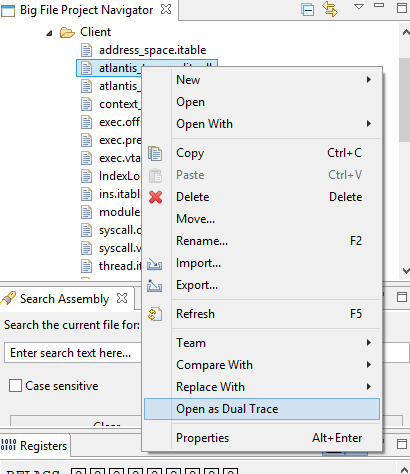
\includegraphics[scale=0.7]{Figures/opendualtracemenu}}
 \caption{Menu Item for opening Dual\_trace}
\label{opendualtracemenu}
\end{figure}

\begin{figure}[H]
\centerline{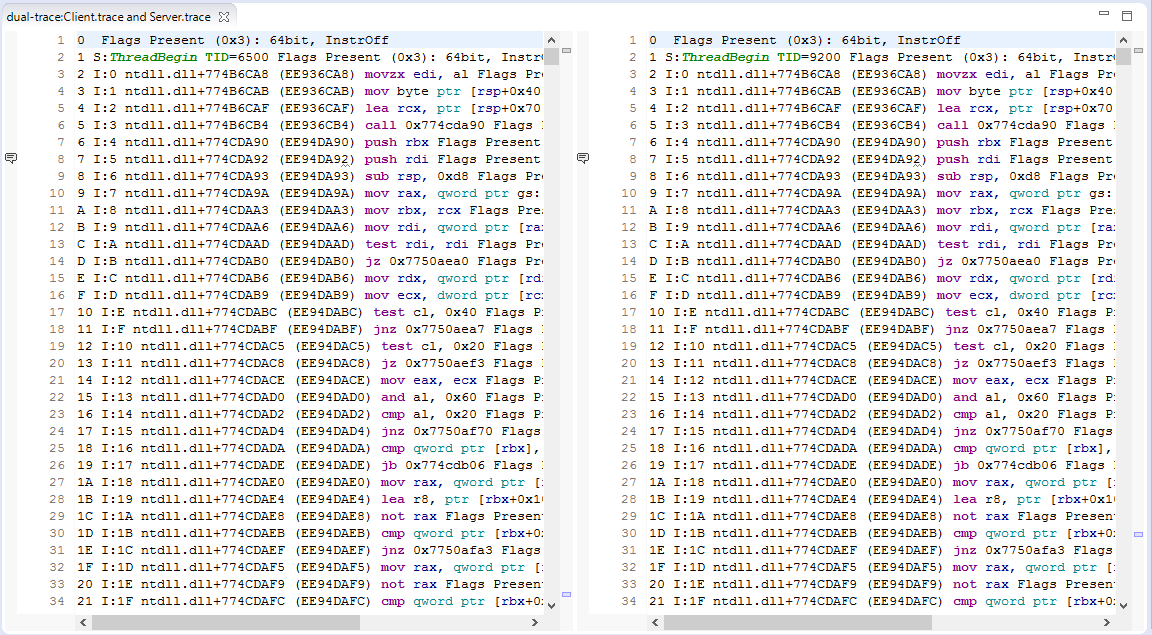
\includegraphics[scale=0.6]{Figures/paralleleditor}}
 \caption{Parallel Editor View}
\label{paralleleditor}
\end{figure}



\section{Identification Features}
I implemented two identification features, one is stream identification for both traces in the dual\_trace, the other is the communication identification. These two features align to the ``stream identification algorithm" and ``communication identification algorithm" designed in Chapter\ref{chapter:alo}. The implementation of these two identification features relies on the existing ``function inspect" feature of Atlantis. The called functions' name can be inspected  by  search of the symbolic name in the executable binary or any DLLs which used by the program at the time when it is traced. By importing the DLLs and executable binary, Atlantis can recognize the function call from the execution trace by the function names. Therefore the corresponding Dlls or executable binaries for both traces in the dual\_trace have to be loaded into Atlantis before conducting the identification.

A new menu ``Dual\_trace Tool" with three menu options is designed for these two identification features. In this menu, two options are for conducting the identification which are ``Stream Identification" and ``Communication Identification" while one is for loading the DLLs and executable binary which is ``Load Library Exports". Currently, the ``Load library export" function can only load libraries for the trace in the active editor. So this item in the menu has to be run twice separately for each trace of the dual\_trace.  Figure\ref{dualtracetoolmenu} shows this new menu in Atlantis. When the user perform any of the identification features, there is the prompt dialog as shown in Figure\ref{methods} which asks the user what communication methods they want to identify from the dual\_trace. This list is provided by the configuration file I mention in Section\ref{functionset}. The user can select one or multiple methods. 

\begin{figure}[H]
\centerline{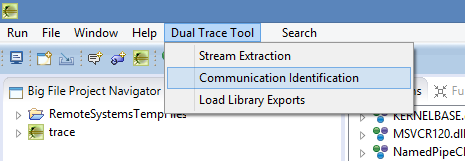
\includegraphics{Figures/dualtracetoolmenu}}
 \caption{Dual\_trace Tool Menu}
\label{dualtracetoolmenu}
\end{figure}

\begin{figure}[H]
\centerline{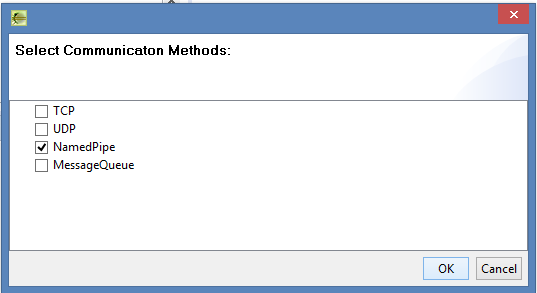
\includegraphics[scale=0.8]{Figures/methods}}
 \caption{Prompt Dialog for Communication Selection}
\label{methods}
\end{figure}

A new view named ``Communication" is designed for presenting the result of the identification of streams and communications. Since the user can have multiple selection for communication methods they concern, the output identification result contains all the identified communications or streams of all the concerned communication methods and the identified results are clustered by methods. There are two sub tables in this view, the left one is for the stream identification result while the left one is for communication identification result. The reason for putting this two result in the same view is for easy access and comparison of the data for the users. Figure\ref{idenview} shows this view with result data in it. Each time when the user rerun the identification features the result in the corresponding table will be refreshed to show only the latest identification result. But the other table will not be affected. For example, if the user run the ``Stream Identification" feature first, the stream identification result will show on the left table of the view. And then the user run the ``communication Identification", the communication identification result will be shown on the right table while the left one still holding the last stream identification result.

\begin{figure}[H]
\centerline{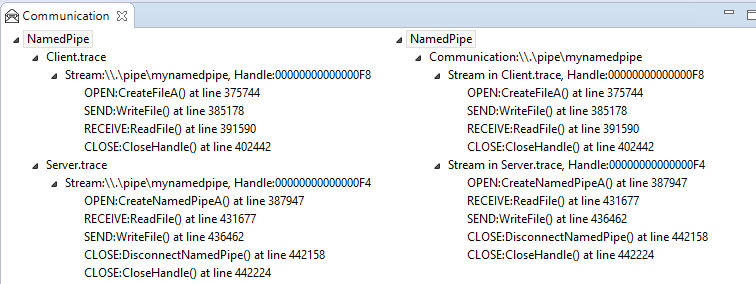
\includegraphics[scale=0.7]{Figures/idenview}}
 \caption{Communication View for Showing Identification Result}
\label{idenview}
\end{figure}

\section{Identification Result View and Result Navigation}
Atlantis is a analysis environment that has various views to allow user access to different information from the trace, such as the memory and register state of the current instruction line. Moreover, these views synchronize automatically with the editor view. These functionality and information also benefit the communication analysis of the dual\_trace. Providing the user a way to navigate from the identified result to the traces in the editors allows them to take advantage of the current existing functionality of Atlantis and make their analysis of the dual\_trace more efficient.

In the result list, each event entry is corresponding to a function call. The functions were called at function call line and all the inputs of the function calls can be recovered from the memory state of this instruction line. The functions returned at the return instruction lines, all the outputs of the function calls can be recovered in the memory state of the the return instruction line. From the event entries, this implementation provide two different ways for the user to navigate back to where the function begins and ends. When the user ``double click" on an entry, it will bring the user to the start line of the function in the corresponding trace editor. When the the right click on the event entry, a prompted menu with the option ``Go To Line of Function End" will show up as in Figure\ref{gotoend}. Clicking on this option will bring the user to the return line of this function in the trace editor. All other views update immediately with this navigation. 

\begin{figure}[H]
\centerline{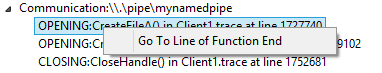
\includegraphics{Figures/gotoend}}
 \caption{Right Click Menu on Event Entry}
\label{idenview}
\end{figure}

Moreover, the ``remove" option as shown in Figure\ref{remove} in the right click menu on the ``stream“ or ``communication" entries is provided for the user to remove the selected ``stream" or ``communication" entry. This provides the user the flexibility to get rid of the data that they don't care.

\begin{figure}[H]
\centerline{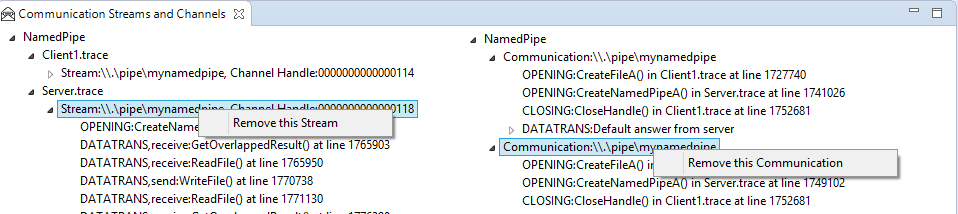
\includegraphics[scale=0.7]{Figures/remove}}
 \caption{Right Click Menu on Event Entry}
\label{remove}
\end{figure}


